\section{速度合成律的失效}\label{sec:02.06}

如图\ref{fig:02.10}~所示,如果在炮车上装有两门相同的大炮,一门向
右,一门向左。如果炮车相对地面静止〔图\ref{fig:02.10a}〕,这时,不论
从地面参考系$K$,还是从炮车参考系$K'$看,同时向左、右发射出
的炮弹的速率都是$v$。如果炮车相对地面以$u$的速率向右匀速运动
〔图\ref{fig:02.10b}〕,从$K$看,按速度合成规律〔式\eqref{eqn:02.03.06}〕,向右的炮
弹速率是$v+u$;向左的炮弹速率是$v-u$。实验也相当精确地证
明了这一点,它表明,速度的合成公式是符合实际的。

我们现在要问:速度合成律对任何情况都成立吗?

\clearpage
\begin{figure}
    \centering
    \subfigure[]{
        \includegraphics{figure/fig02.10a}
        \label{fig:02.10a}
    }
    \hspace{2em}
    \subfigure[]{
        \centering
        \includegraphics{figure/fig02.10b}
        \label{fig:02.10b}
    }
    \caption{速度的合成}
    \label{fig:02.10}
\end{figure}

\begin{figure}
    \centering
    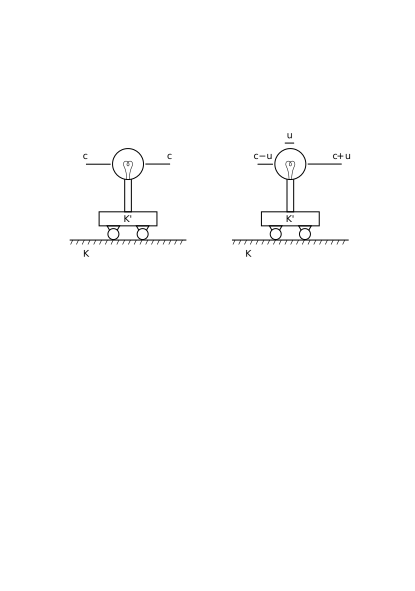
\includegraphics{figure/fig02.11}
    \caption{光的速度合成}
    \label{fig:02.11}
\end{figure}

再考虑一个如图\ref{fig:02.11}~所示的实验,这里仅把大炮改为灯泡,
灯泡发出的光与炮弹相当,光相对于灯泡的速率是$c$。根据速度合
成律,当灯泡相对于地面以速率$u$向右匀速运动时,则向右发出的
光对于地面参考系$K$的速率应是$c+u$,而向左发出的光对于$K$的
速率应是$c-u$。这个结果对吗?现在我们举一些显而易见的例
子,来说明这个结果是不正确的。

上述实验是把速度合成律应用到光传播的现象中去。根据光
学知识,我们知道,一个物体$A$之所以能被看到,是由于从物体
$A$发出的光(或从它反射的光)传到了我们的眼睛。例如,在图2-12
中,1投球,2接球。2看到球$A$,是由于球$A$发出的光到达2。如果
光速为$c$,1到2之间距离为$L$,并且1即将投球的时刻为$t=0$,则
2看到1即将投球的时刻为
\begin{equation*}
    t_{2\text{投}}=\frac{L}{c}
\end{equation*}